\chapter{Dziedzina problemu}

\begin{figure}
 \centering
 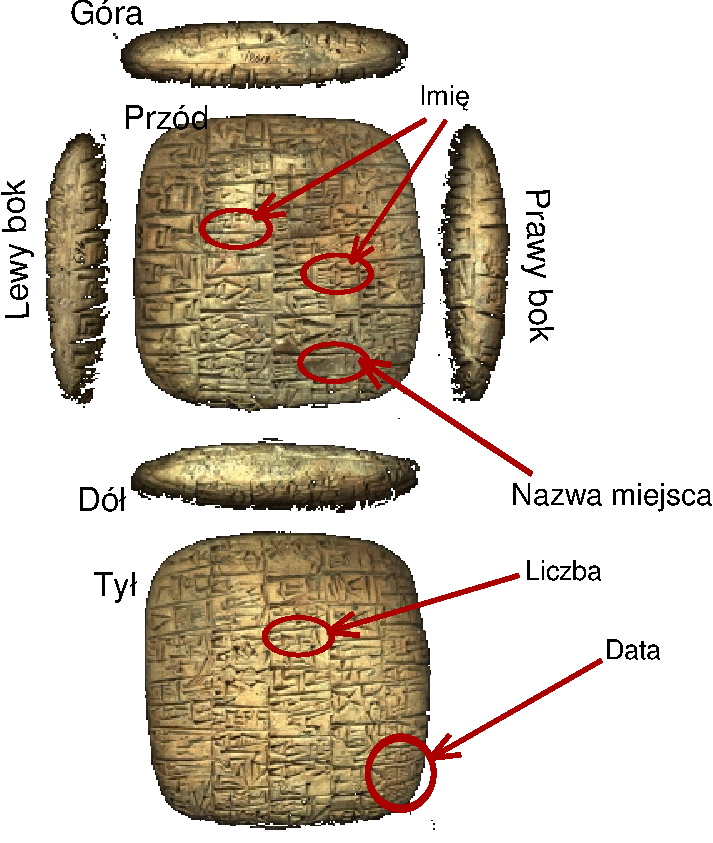
\includegraphics[bb=0 0 342 405]{../diagramy/tabliczka.pdf}
 % tabliczka.pdf: 342x405 pixel, 72dpi, 12.06x14.29 cm, bb=0 0 342 405
 \caption{Gliniana tabliczka - struktura}
\end{figure}

\begin{figure}
 \centering
 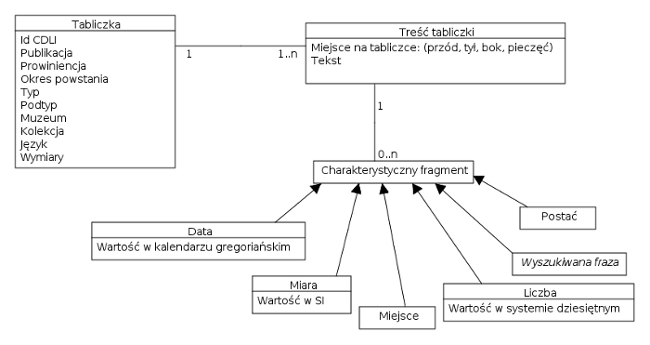
\includegraphics[width=500px,bb=0 0 650 345]{../diagramy/Model-dziedziny.png}
 % Model-dziedziny.png: 650x345 pixel, 72dpi, 22.93x12.17 cm, bb=0 0 650 345
 \caption{Co powinna zawierać tabliczka w formie elektronicznej}
\end{figure}

Głównym pojęciem jest tabliczka. Ma ona swoje metadane i treść. Tabliczka jest rozumiana dwojako - jako fizyczna tabliczka gliniana
zapisana klinami lub jako tabliczka w formie cyfrowej zapisana odczytami. Może ona zawierać elementy znaczące takie jak imię jakiejś 
osoby, liczba, jednostka (np. przy opisywaniu wypłat), miejsce, data, imię bóstwa. Część tych elementów da się przetłumaczyć na 
współczesny język (np. jednostki przeliczyć na SI, datę na datę liczbową BC). Gliniane tabliczki są zapisywane z różnych stron 
(od góry, z przodu, z tyłu itp). Poza tym zawierają pieczęcie. 

Sumerolodzy rozpoznają tabliczki po publikacjach - wiedzą mniej więcej o co chodzi jak widzą publikację.

Odczyty zawarte w cyfrowym zapisie tabliczki są wariantem tłumaczenia z klinów. W cyfrowej wersji nie ma klinów, stąd też możliwe
są pomyłki w tłumaczeniach, które ciężko zweryfikować. Są też uszkodzone fragmenty, które zostały cyfrowo zapisane w najróżniejszej
formie.

Sumerolodzy oczekują możliwości wyszukiwania po metadanych, po treści tabliczki (odczyty) i po możliwych innych tłumaczeniach (po klinach).
W pierwszej wersji języka implementujemy tylko wyszukiwanie po odczytach.